\documentclass[12pt]{article}
\usepackage[spanish]{babel}
\usepackage[utf8]{inputenc}
\usepackage{amsmath}
\usepackage{graphicx}
\usepackage{pdfpages}
\usepackage{listings}

\begin{document}

\begin{titlepage}

\newcommand{\HRule}{\rule{\linewidth}{0.5mm}}

\center

\textsc{\LARGE Universidad de Buenos Aires}\\[1.5cm]

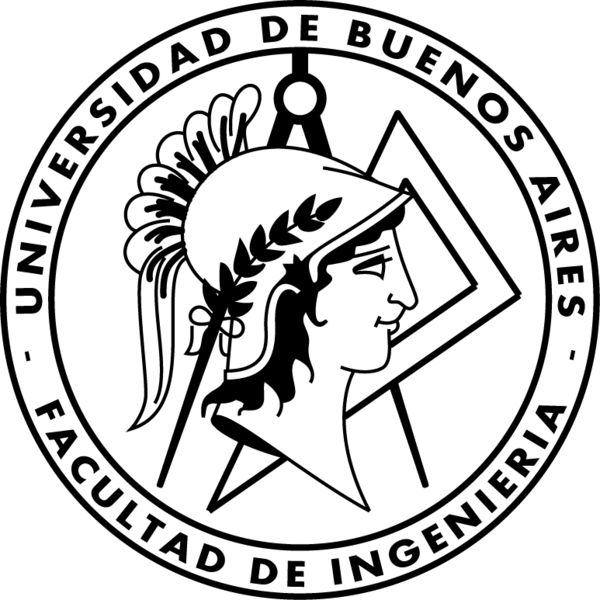
\includegraphics{docs/images/logo-fiuba.png}\\[1cm]

\textsc{\Large Facultad de Ingeniería}\\[0.5cm]
\textsc{\large (75.31) Teoría de Lenguaje}\\[0.5cm]
{\large 1\textsuperscript{er} Cuatrimestre 2015}\\[0.5cm]

\HRule \\[0.4cm]
{ \huge \bfseries Trabajo Práctico Integrador}\\[0.4cm]
\HRule \\[1.5cm]

\large Andrés Arana, P.86203

\vfill

\end{titlepage}

\begin{abstract}

El presente informe se sumarizan las soluciones a los diferentes problemas
planteados para los lenguajes como trabajo integrador de la materia (75.31)
Teoría de Lenguaje.

\end{abstract}

\tableofcontents

\clearpage

\section{Ejercicio Integrador}

\subsection{Referencias externas}

\subsection{Ejemplo de ejecución}

\subsection{Hilos}

\subsection{Evaluación perezoza}

\subsection{Parámetros}

\subsection{Mensajes}

\subsection{Celdas de memoria}

\subsection{Abstracción de datos}

\subsection{Más abstracción de datos}

\clearpage
\appendix

\section{Enunciado ejercicio Integrador}

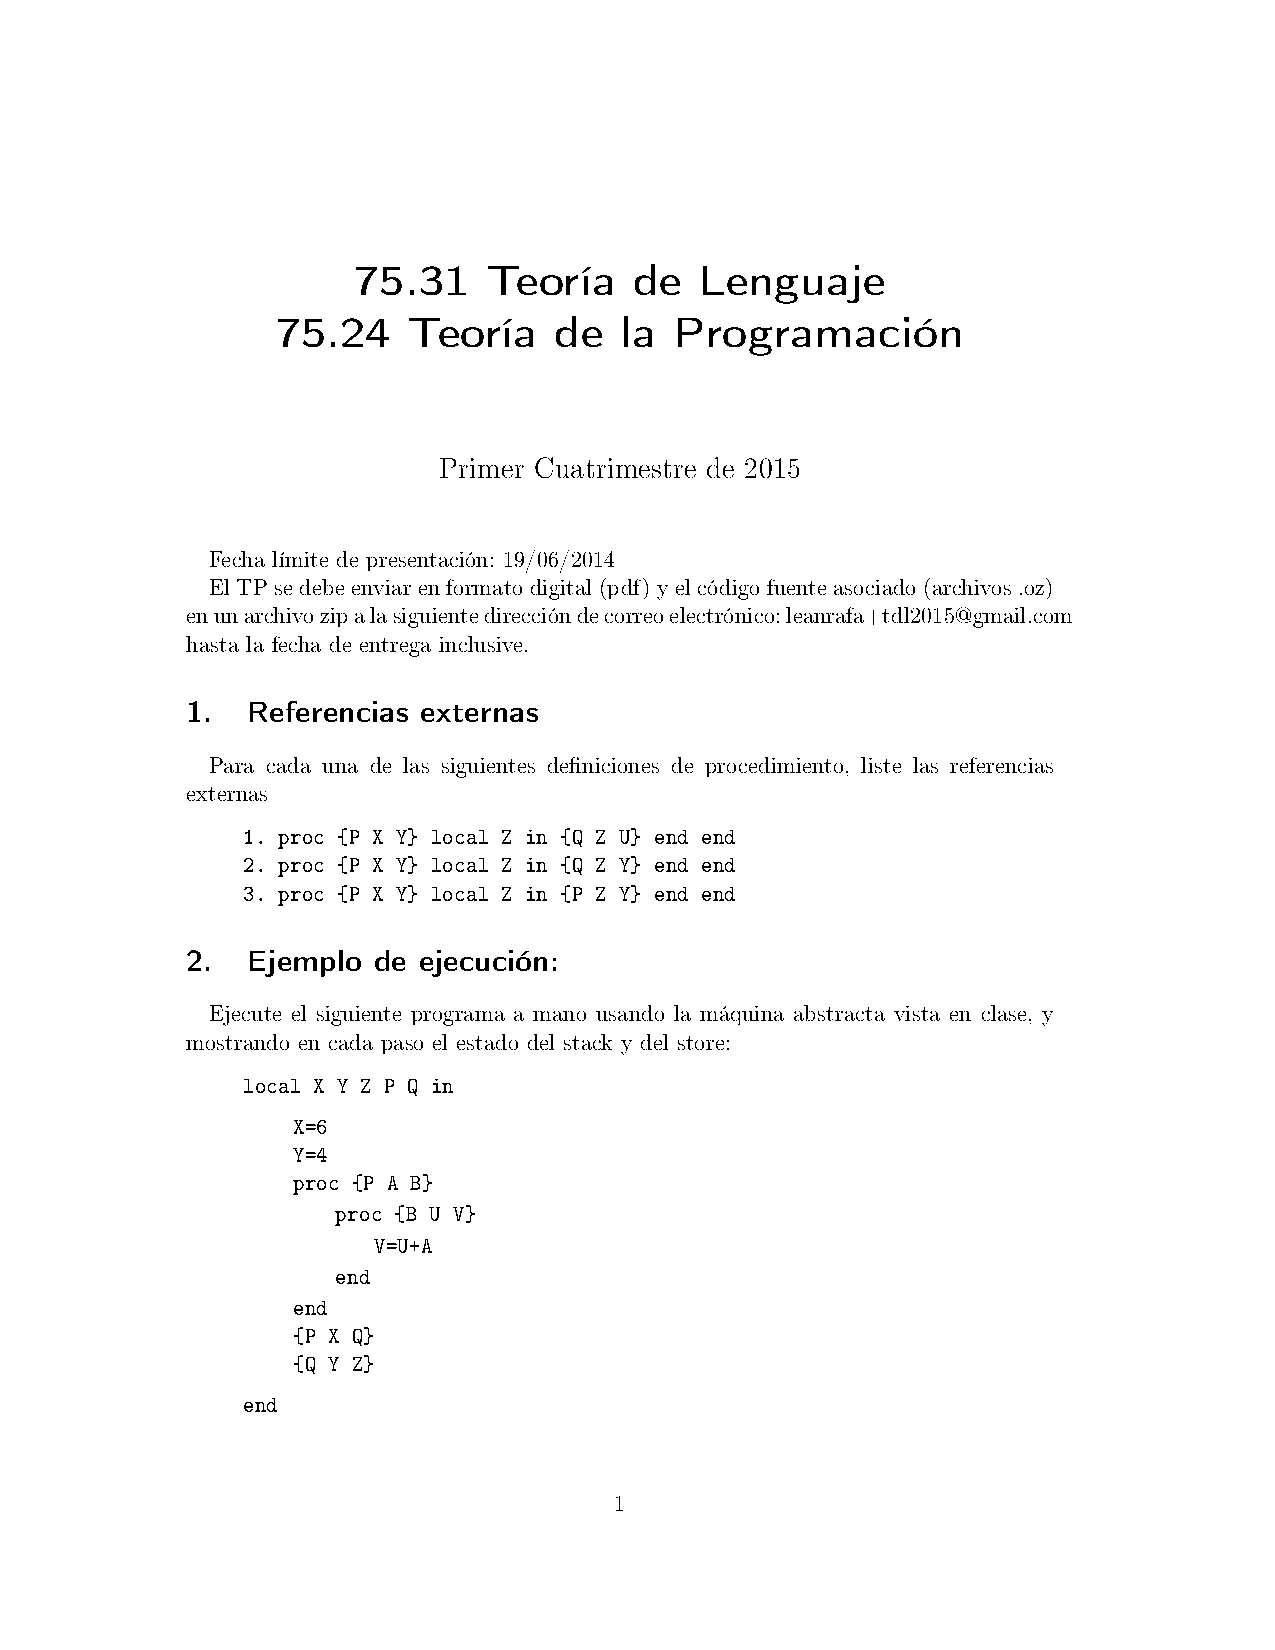
\includepdf[pages=-,scale=.75,pagecommand={}]{docs/enunciados/ejercicios.pdf}

\end{document}
